% =====================================================================
% Governance-Aware Routing for Networked LLM Applications
% JNCA-oriented bounded systems manuscript
% =====================================================================
\documentclass[10pt,journal,compsoc]{IEEEtran}

\usepackage[utf8]{inputenc}
\usepackage[T1]{fontenc}
\usepackage{textcomp}
\ifCLASSOPTIONcompsoc
  \usepackage[nocompress]{cite}
\else
  \usepackage{cite}
\fi
\usepackage{amsmath,amssymb}
\usepackage{booktabs}
\usepackage{array}
\usepackage{graphicx}
\usepackage{xcolor}
\usepackage{pifont}
\usepackage{url}
\usepackage[hidelinks]{hyperref}
\def\UrlBreaks{\do\/\do-\do\_\do\.\do\:}
\Urlmuskip=0mu plus 1mu\relax

\newcommand{\cmark}{\textcolor{green!55!black}{\ding{51}}}
\newcommand{\xmark}{\textcolor{red!70!black}{\ding{55}}}
\newcommand{\Ours}{\textbf{Ours}}
\graphicspath{{figures/}}
\renewcommand{\arraystretch}{1.12}

\title{Governance-Aware Routing for Networked LLM Applications:\\
A Kubernetes Gateway Control Plane for Cost, Declared Sovereignty, and Budget Trade-offs}

\author{Anonymous~Authors%
\IEEEcompsocitemizethanks{\IEEEcompsocthanksitem Manuscript prepared for
anonymous review.}}
\markboth{Journal of Network and Computer Applications,~Submission Manuscript}%
{Anonymous Authors: Governance-Aware Routing for Networked LLM Applications}

\begin{document}

\IEEEtitleabstractindextext{%
\begin{abstract}
Networked LLM applications increasingly route requests through gateway
infrastructures to multiple model providers, creating operational trade-offs
between cost, latency, quality, budget pressure, workload ownership, and
declared data-residency constraints. We present a Kubernetes-native gateway
control plane that makes these routing decisions explicit and auditable. The
system represents providers, models, budgets, routing policies, reports, and
declared residency constraints as Kubernetes resources; filters non-compliant
candidates using declared policy metadata; and ranks feasible candidates using
cost, quality, latency, reliability, and budget-pressure signals implemented by
the operator and experiment engines. We evaluate the approach in a bounded
two-provider testbed while separating measured, cached, and simulated evidence.
In cached replays of previously collected real API calls, the policy reduces
cost by 70.8\% relative to an always-premium baseline under the evaluated
workload mix and committed catalog prices; the absolute total is 0.011 EUR over
40 prompts, so it is evidence of routing behavior rather than deployment-scale
savings. A 30-repetition uncached run confirms stable cost separation under the
fixed matrix but also a measurable latency increase. On objective GSM8K/MMLU
tasks, the same cost-aware policy lowers exact-match accuracy from 65.4\% to
47.2\%, showing that static quality priors are insufficient for
correctness-critical workloads. Simulated policy scenarios prevent configured
violations by construction under declared metadata while exposing cost and
availability trade-offs. An ephemeral Kubernetes integration run verifies
gateway telemetry, workload attribution, and shadow-AI evidence ingestion. The
result is a reproducible control-plane framework for trade-off visibility and
auditability in cloud-native LLM routing.
\end{abstract}

\begin{IEEEkeywords}
LLM gateways, cloud-native applications, Kubernetes operators, model routing,
FinOps, declared data sovereignty, AI governance, policy-as-code, LLM
evaluation.
\end{IEEEkeywords}}

\maketitle
\IEEEdisplaynontitleabstractindextext
\IEEEpeerreviewmaketitle

% =====================================================================
\IEEEraisesectionheading{\section{Introduction}\label{sec:introduction}}
\IEEEPARstart{A}{ typical enterprise LLM application is a networked service:}
user requests enter through an API gateway, are attributed to a Kubernetes
workload, and are forwarded to one of several managed model endpoints. The
routing choice affects cost, latency, declared data-residency constraints, team
budgets, and auditability. This makes LLM routing a networked application
governance problem rather than only a model-selection problem.

Three operational problems recur. First, model spend is often opaque: gateway
logs expose requests, but teams need attribution by namespace, application,
team, provider, and model. Second, declared data-residency and sensitive-data
policies are rarely embedded in the routing plane; they are often checked after
the fact, if at all. Third, budget pressure is operational: when a namespace is
near a monthly cap, the platform should expose whether cheaper feasible models,
stricter guardrails, or blocking are appropriate.

We study these problems in a bounded systems artifact: a Kubernetes operator and
gateway-adjacent experiment harness for governance-aware LLM routing. The
artifact does not claim legal certification of provider residency, broad
deployment validation, or universal quality guarantees. Instead, it provides a
reproducible framework for making routing trade-offs visible and auditable.

\paragraph{Contributions.}
This paper makes four contributions:
\begin{enumerate}
  \item A Kubernetes-native gateway control-plane architecture for
        governance-aware LLM routing in networked applications, using CRDs,
        reconciliation loops, telemetry collectors, and workload-level
        attribution.
  \item A declared-policy routing formulation that filters non-compliant model
        candidates before scoring feasible candidates by cost, expected quality,
        latency, reliability, and budget pressure.
  \item A reproducible evidence methodology that separates \textbf{MEASURED},
        \textbf{CACHED}, and \textbf{SIMULATED} evidence across cost, quality,
        latency, declared-policy compliance, budget behavior, and integration
        verification.
  \item A methodological result showing that open-ended LLM-as-judge quality can
        be misleading for objective tasks: GSM8K/MMLU exact-match accuracy drops
        under aggressive cost routing, motivating premium pinning or task-type
        guardrails for correctness-critical workloads.
\end{enumerate}

% =====================================================================
\section{Related Work}

\subsection{LLM Routing and Cascades}
FrugalGPT~\cite{chen2023frugalgpt}, Hybrid LLM~\cite{ding2024hybridllm},
RouteLLM~\cite{ong2024routellm}, AutoMix~\cite{aggarwal2024automix}, and recent
bandit or mixture routers~\cite{li2025llmbandit,wang2025mixllm} reduce cost by
selecting models based on predicted difficulty, confidence, or learned
preference data. These methods are complementary to this work. Our focus is not
to outperform learned routers; it is to expose Kubernetes-native governance
constraints, workload attribution, budget state, and audit traces around the
routing decision. The heuristic difficulty proxy in the artifact is not a
reproduction of RouteLLM or Hybrid LLM and is not used as a main comparative
claim.

\subsection{Gateways, Operators, and Telemetry}
Gateway layers such as Envoy AI Gateway~\cite{envoyaigateway}, Envoy
Gateway~\cite{envoygateway}, and LiteLLM~\cite{litellm} provide operational
entry points for model traffic. Kubernetes operators and CRDs~\cite{
kubernetesoperators,kubernetescrd} provide a natural control-plane abstraction:
desired state is declared, controllers reconcile status, and decisions are
visible through Kubernetes APIs. OpenTelemetry~\cite{opentelemetry} and eBPF
systems such as Tetragon~\cite{tetragon} provide the telemetry substrate for
usage attribution and direct-egress evidence.

\subsection{FinOps, Policy, and Evaluation}
FinOps and Kubernetes cost-allocation systems~\cite{finopsframework,opencost}
motivate per-team spend visibility. AI governance frameworks and regulations
\cite{nistairmf2023,nistgenai2024,owaspllm2025,iso42001,euaiact2024,gdpr2016}
motivate auditable controls, but they do not by themselves define gateway-level
routing mechanisms. Evaluation work such as HELM~\cite{liang2022helm},
GSM8K~\cite{cobbe2021gsm8k}, MMLU~\cite{hendrycks2021mmlu}, G-Eval
\cite{liu2023geval}, and LLM-as-judge studies~\cite{zheng2023judge} motivates
separating open-ended quality proxies from objective correctness.

\begin{table}[t]
\centering
\caption{Capability positioning. The comparison is scoped to capabilities
evaluated or explicitly provided by the cited systems, not all possible
extensions.}
\label{tab:positioning}
\begin{tabular}{lccccc}
\toprule
Capability & FrugalGPT & Hybrid & RouteLLM & LiteLLM & \Ours \\
\midrule
Cost-aware model selection & \cmark & \cmark & \cmark & \cmark & \cmark \\
Kubernetes CRDs/status & \xmark & \xmark & \xmark & \xmark & \cmark \\
Workload attribution & \xmark & \xmark & \xmark & partial & \cmark \\
Declared-residency filtering & \xmark & \xmark & \xmark & partial & \cmark \\
Budget phase integration & \xmark & \xmark & \xmark & \xmark & \cmark \\
Evidence separation & \xmark & \xmark & \xmark & \xmark & \cmark \\
\bottomrule
\end{tabular}
\end{table}

% =====================================================================
\section{System Design}

\subsection{Control-Plane Resources}
The operator models gateway governance with Kubernetes custom resources:
\emph{AIProvider} declares provider metadata and pricing, \emph{AIModel}
declares model/provider association and workload ownership, \emph{AIGateway}
declares telemetry collection, \emph{AISovereigntyPolicy} declares allowed and
forbidden zones plus sensitive-data rules, \emph{AIBudgetPolicy} declares
budget thresholds and optional guarded fallback, \emph{AIRoutingPolicy} emits
recommendations, \emph{AIFinOpsReport} summarizes spend, findings, and routing
scores, and \emph{AIQualityGate} evaluates candidate quality from golden
evidence.

The operator enforces declared technical routing policies; it does not
independently certify provider legal compliance or contractual data residency.
Provider zones are catalog metadata. A compliant decision therefore means
``compliant with configured declared metadata,'' not proof of actual data
movement.

\subsection{Routing Formulation}
The control plane separates hard constraints from soft scoring. A request first
defines a feasible set of candidate models. Declared-policy filtering removes
candidates whose provider metadata violates the active policy. Remaining
candidates are ranked by cost, quality, latency, reliability, and budget signals.

\begin{figure}[t]
\small
\begin{verbatim}
Algorithm 1: Governance-aware LLM routing
Input: request metadata, catalog, policy, budget, weights
Output: selected model or block decision
1  candidates <- catalog models allowed for workload
2  rejected <- apply declared-policy filter(candidates, policy)
3  if candidates is empty: block and emit rejection reasons
4  compute cost from token estimate or observed usage
5  compute quality prior/evidence signal
6  compute latency and reliability from telemetry if available
7  compute budget-pressure signal from budget phase/usage
8  normalize features and score feasible candidates
9  select best candidate subject to guardrails
10 emit decision trace, scores, and rejected candidates
\end{verbatim}
\caption{Algorithmic structure of the control-plane routing decision. Evidence:
IMPLEMENTED.}
\label{fig:algorithm}
\end{figure}

The experiment harness uses a transparent argmin score:
\begin{equation}
S(m)=\alpha C_m(1+\epsilon B)+\beta Q_m+\gamma L_m+\delta R_m,
\end{equation}
where $C_m$ is cost normalized to the premium model, $B$ is budget pressure,
$Q_m$ is expected quality loss relative to premium, $L_m$ is latency prior
penalty, and $R_m$ is residual declared-policy risk after filtering. The default
harness weights are $\alpha=1.0$, $\beta=1.5$, $\gamma=0.3$, $\delta=0.5$, and
$\epsilon=1.0$.

The operator runtime scoring engine is different and is reported as
implementation status rather than conflated with the harness. It computes a
higher-is-better score in $[0,1]$ per namespace/application/model/provider:
\begin{equation}
0.40\,CostScore + 0.30\,QualityScore + 0.20\,LatencyScore +
0.10\,ReliabilityScore.
\end{equation}
Cost and latency use inverse min--max normalization over observed groups;
quality is a static catalog tier prior; reliability is $1-errors/requests$.
Sovereignty is a hard gate: a non-compliant model receives score 0 regardless of
soft terms.

\subsection{Quality and Budget Engines}
The quality subsystem has three layers. The pure \emph{qualityengine} computes a
0--100 composite score from correctness, reliability, latency, semantic, and
judge dimensions; missing weighted evidence yields \emph{insufficient-data}
rather than a fabricated score. The \emph{qualitystats} package adds
non-inferiority testing and hysteresis. The \emph{qualityeval} pipeline runs
golden prompts against the production gateway and serializes evidence for the
pure engine. In this paper, the open-ended quality result uses the experiment
harness judge scores; the operator quality gate is implemented but not claimed
as a main evaluated result.

The budget engine maps projected monthly spend to phases
\emph{WithinBudget}, \emph{Warning}, \emph{Critical}, and \emph{Exceeded}.
Actions are advisory unless the user explicitly configures guarded fallback
actuation against Envoy AI Gateway routes. The reported budget result is a
simulated pressure scenario over existing workload rows.

\subsection{Telemetry and Shadow-AI Evidence}
The Envoy AI Gateway collector reads OpenTelemetry Prometheus metrics for token
usage and request duration, then attributes usage to Kubernetes namespaces and
applications using request headers or AIModel catalog metadata. Shadow-AI
evidence is gateway-independent: eBPF/Tetragon-derived egress observations are
loaded from a ConfigMap and classified against the same declared-policy engine.
This detects direct egress to known LLM endpoints; it does not itself block
traffic.

% =====================================================================
\section{Methodology}

\subsection{Evidence Labels}
\begin{table}[t]
\centering
\caption{Evidence map used in the revised paper.}
\label{tab:evidence}
\begin{tabular}{p{0.11\linewidth}p{0.27\linewidth}p{0.18\linewidth}p{0.24\linewidth}}
\toprule
RQ & Main claim & Evidence & Scope/limitation \\
\midrule
RQ1 & Cost and routing distribution & CACHED + MEASURED N=30 & Two-provider harness; catalog-dependent \\
RQ2 & Open-ended judge-assessed quality & CACHED & Judge proxy only \\
RQ2b & Objective accuracy & CACHED & GSM8K/MMLU subset \\
RQ3 & Latency and overhead & CACHED + MEASURED N=30 & Provider variance not isolated \\
RQ4 & Declared-policy trade-offs & SIMULATED & Declared metadata, not legal certification \\
RQ5 & Budget behavior & SIMULATED & One pressure scenario \\
\bottomrule
\end{tabular}
\end{table}

\subsection{Workloads and Data}
\begin{table}[t]
\centering
\caption{Workload construction.}
\label{tab:workloads}
\begin{tabular}{p{0.26\linewidth}p{0.18\linewidth}p{0.12\linewidth}p{0.18\linewidth}p{0.16\linewidth}}
\toprule
Dataset/workload & Source & Prompts & Task type & Used for \\
\midrule
W1 HR chatbot & Author-created & 10 & sensitive chat & RQ1--RQ5 \\
W2 RAG docs & Author-created & 10 & document QA & RQ1--RQ5 \\
W3 dev assistant & Author-created & 10 & code/explanation & RQ1--RQ5 \\
W4 analytical agent & Author-created & 10 & analytical QA & RQ1--RQ5 \\
GSM8K subset & Public~\cite{cobbe2021gsm8k} & 250 & math exact match & RQ2b \\
MMLU subset & Public~\cite{hendrycks2021mmlu} & 250 & multiple choice & RQ2b \\
\bottomrule
\end{tabular}
\end{table}

The main matrix is a compact coverage-oriented workload set, not a production
trace. Synthetic prompts were selected deterministically to cover sensitive HR,
document QA, developer assistance, and analytical-agent cases. Public benchmark
subsets provide objective ground truth for accuracy analysis. All paths in the
artifact are repository-relative; provider credentials and secrets are not
included.

\subsection{Strategies and Metrics}
The main manuscript reports strategies whose evaluated rows do not rely on a
stubbed model: B1 premium-static, B4 static namespace policy, B5 budget hard
block, and B6 proposed policy. We exclude earlier B2/B3/B7 rows from the main
figures because some historical rows selected a modeled stub. Metrics are total
cost, cost per request, cost per token, route distribution, open-ended judge
score, exact-match accuracy, latency, configured-policy violations, served and
blocked requests, and budget overrun.

The committed catalog prices are used as a reproducible price snapshot. Absolute
cost values may change with provider pricing; relative conclusions are
catalog-dependent.

% =====================================================================
\section{Results}

\subsection{Integration Verification: Telemetry and Attribution}
An ephemeral Kubernetes integration run verifies that the operator can ingest
Envoy AI Gateway telemetry, attribute token usage to workloads, create report
status, and ingest shadow-AI direct-egress evidence. The integration run is used
as systems verification only. It is not a production security evaluation and is
not used to claim live prevention of bypass traffic.

\subsection{RQ1: Cost and Routing Distribution}
\begin{figure}[t]
\centering
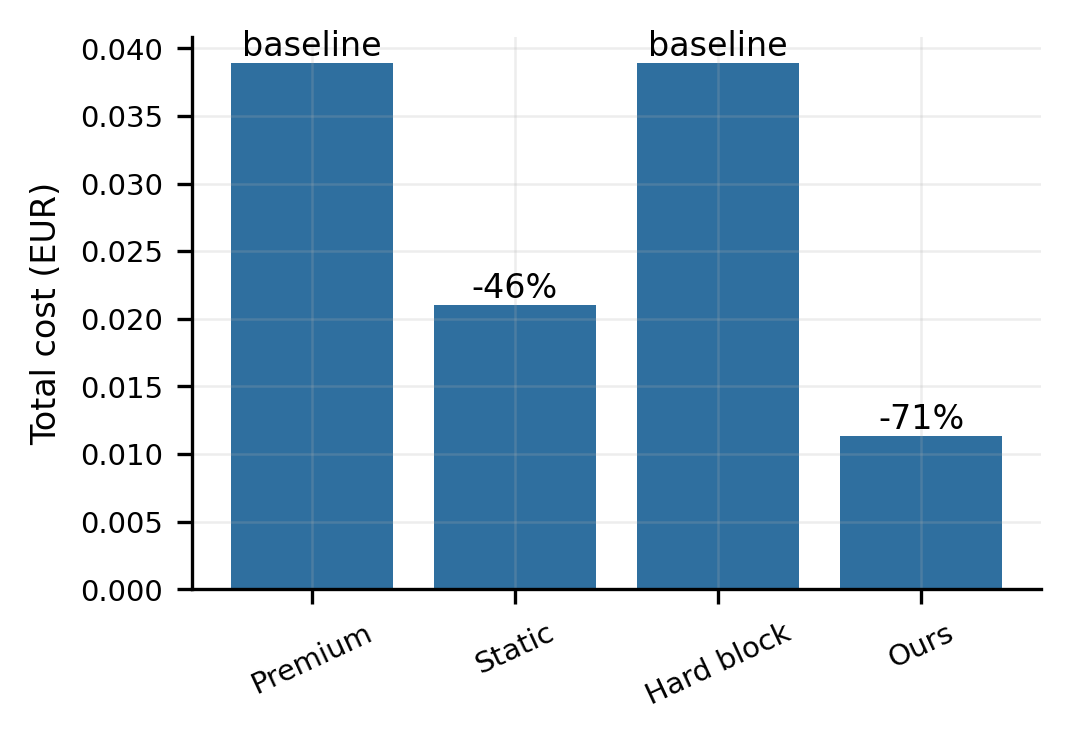
\includegraphics[width=0.95\linewidth]{fig2_cost_by_strategy.png}
\caption{CACHED: total replay cost over the 40-prompt workload matrix.}
\label{fig:cost}
\end{figure}

In the cached replay, \Ours{} costs 0.011353 EUR over 40 prompts versus 0.038930
EUR for premium-static, a 70.8\% reduction under the evaluated workload mix.
Reported per 1,000 requests, this is 0.284 EUR for \Ours{} versus 0.973 EUR for
premium-static. The absolute total is small, so the result demonstrates that the
control plane materially changes route selection under the catalog; it does not
quantify production savings. The \Ours{} route distribution is 30/40
\texttt{gpt-4o-mini} and 10/40 \texttt{mistral-large}; premium-static routes all
40 prompts to \texttt{gpt-4o}.

\subsection{RQ2: Open-Ended Judge-Assessed Quality}
\begin{figure}[t]
\centering
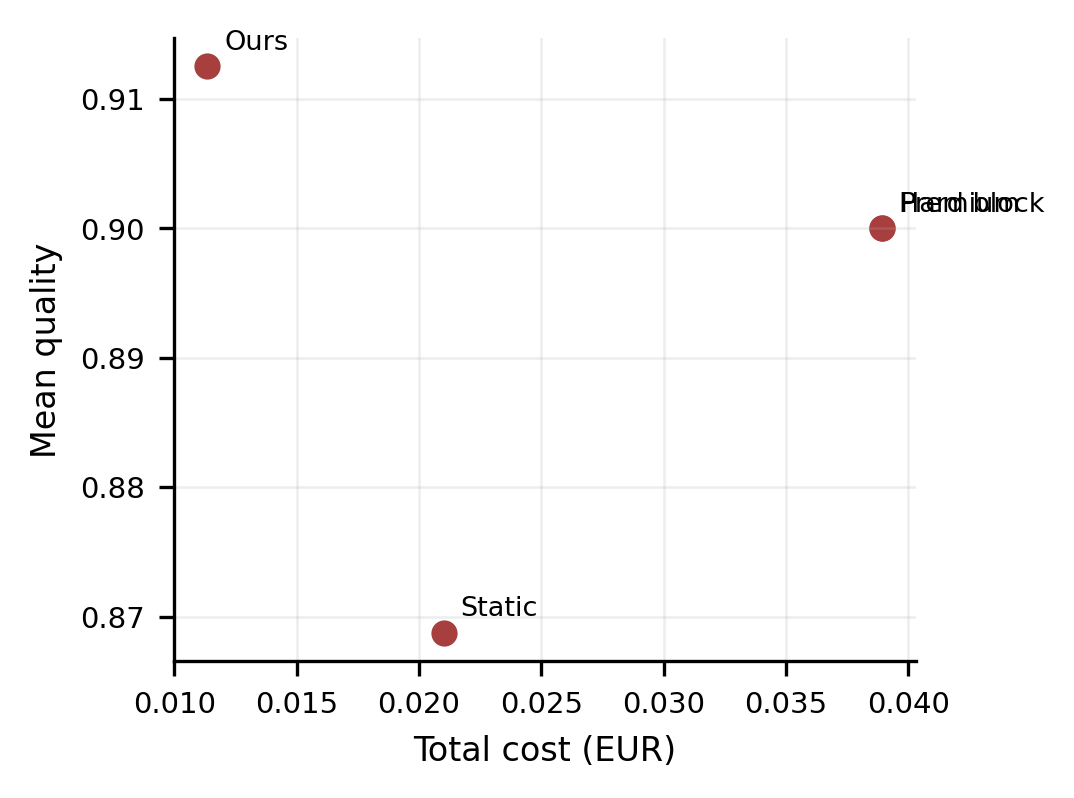
\includegraphics[width=0.95\linewidth]{fig3_quality_vs_cost.png}
\caption{CACHED: cost versus open-ended LLM-as-judge quality. The judge score is
a proxy and should not be interpreted as objective correctness.}
\label{fig:qcost}
\end{figure}

Open-ended judge-assessed quality remains comparable in the evaluated prompt set:
\Ours{} has mean normalized score 0.9125, premium-static 0.9000, and pairwise
win rate 50.0\% over 40 comparisons. We do not interpret this as superiority or
general quality guarantees. Inter-judge agreement is weak-to-moderate
($\kappa=0.403$, Krippendorff $\alpha=0.386$, $n=120$), so judge quality is a
bounded proxy.

\subsection{RQ2b: Objective Accuracy and Failure Analysis}
\begin{table}[t]
\centering
\caption{CACHED: objective benchmark result and task-type guardrail
recomposition.}
\label{tab:objective}
\begin{tabular}{lccc}
\toprule
Policy & Accuracy & Cost (EUR) & p95 latency \\
\midrule
Premium-static & 65.40\% & 0.116388 & 764 ms \\
Cost-aware & 47.20\% & 0.007286 & 891 ms \\
Objective-premium guardrail & 65.40\% & 0.116388 & 764 ms \\
\bottomrule
\end{tabular}
\end{table}

On 500 public GSM8K/MMLU items, \Ours{} lowers cost by selecting cheaper models
but reduces exact-match accuracy from 65.4\% to 47.2\%. This failure is central:
static catalog quality priors and minimum-quality thresholds are insufficient
for correctness-critical tasks. The simple guardrail ``objective tasks use
premium'' restores the measured premium outcome by construction over the same
items, at premium cost. Judge-vs-truth analysis over 300 objective items shows
that 81.1\% of incorrect answers are still rated acceptable ($\geq3$), explaining
why open-ended judge scores cannot replace exact-match evaluation.

\subsection{RQ3: Latency Distribution and Routing Overhead}
\begin{figure}[t]
\centering
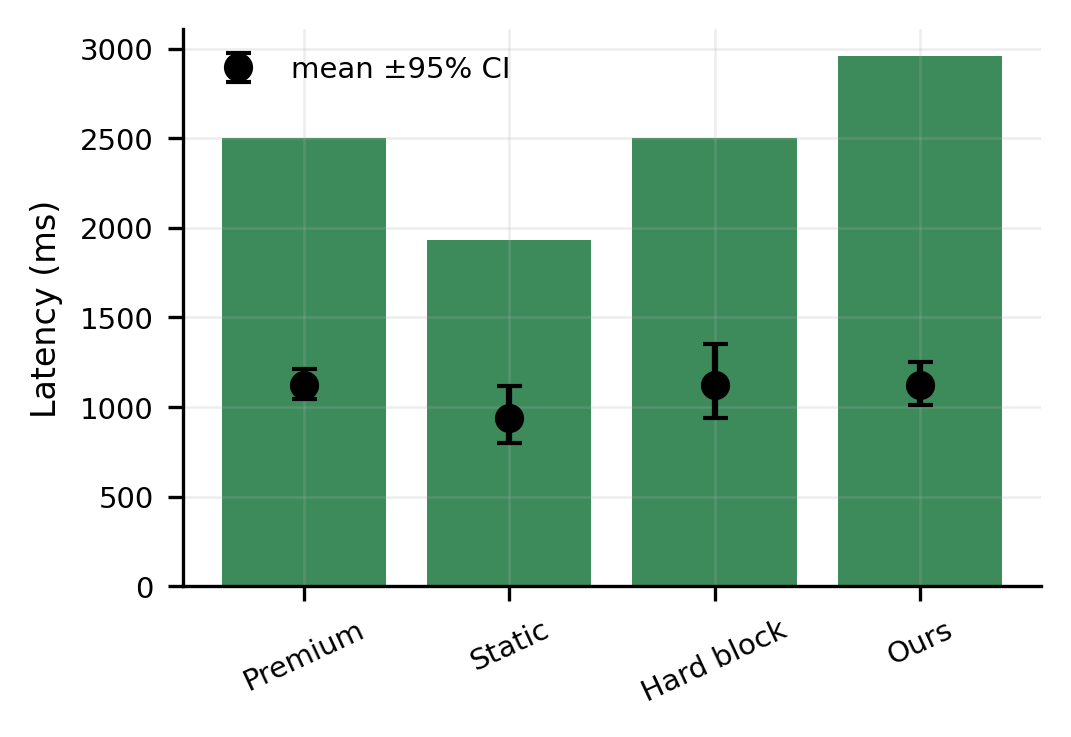
\includegraphics[width=0.95\linewidth]{fig4_latency.png}
\caption{CACHED: p95 latency bars and mean latency confidence intervals over the
main workload rows.}
\label{fig:latency}
\end{figure}

Cost-aware routing increases latency because it changes the provider/model mix.
In the cached matrix, \Ours{} has mean latency 1509.95 ms and p95 3475 ms,
compared with premium-static mean 1125.97 ms and p95 2494 ms. Routing-decision
overhead remains small in the harness (10.83 microseconds on average for
\Ours{}), but end-to-end latency is operationally important.

\subsection{RQ4: Cost, Availability, and Quality Under Declared Policy}
\begin{figure}[t]
\centering
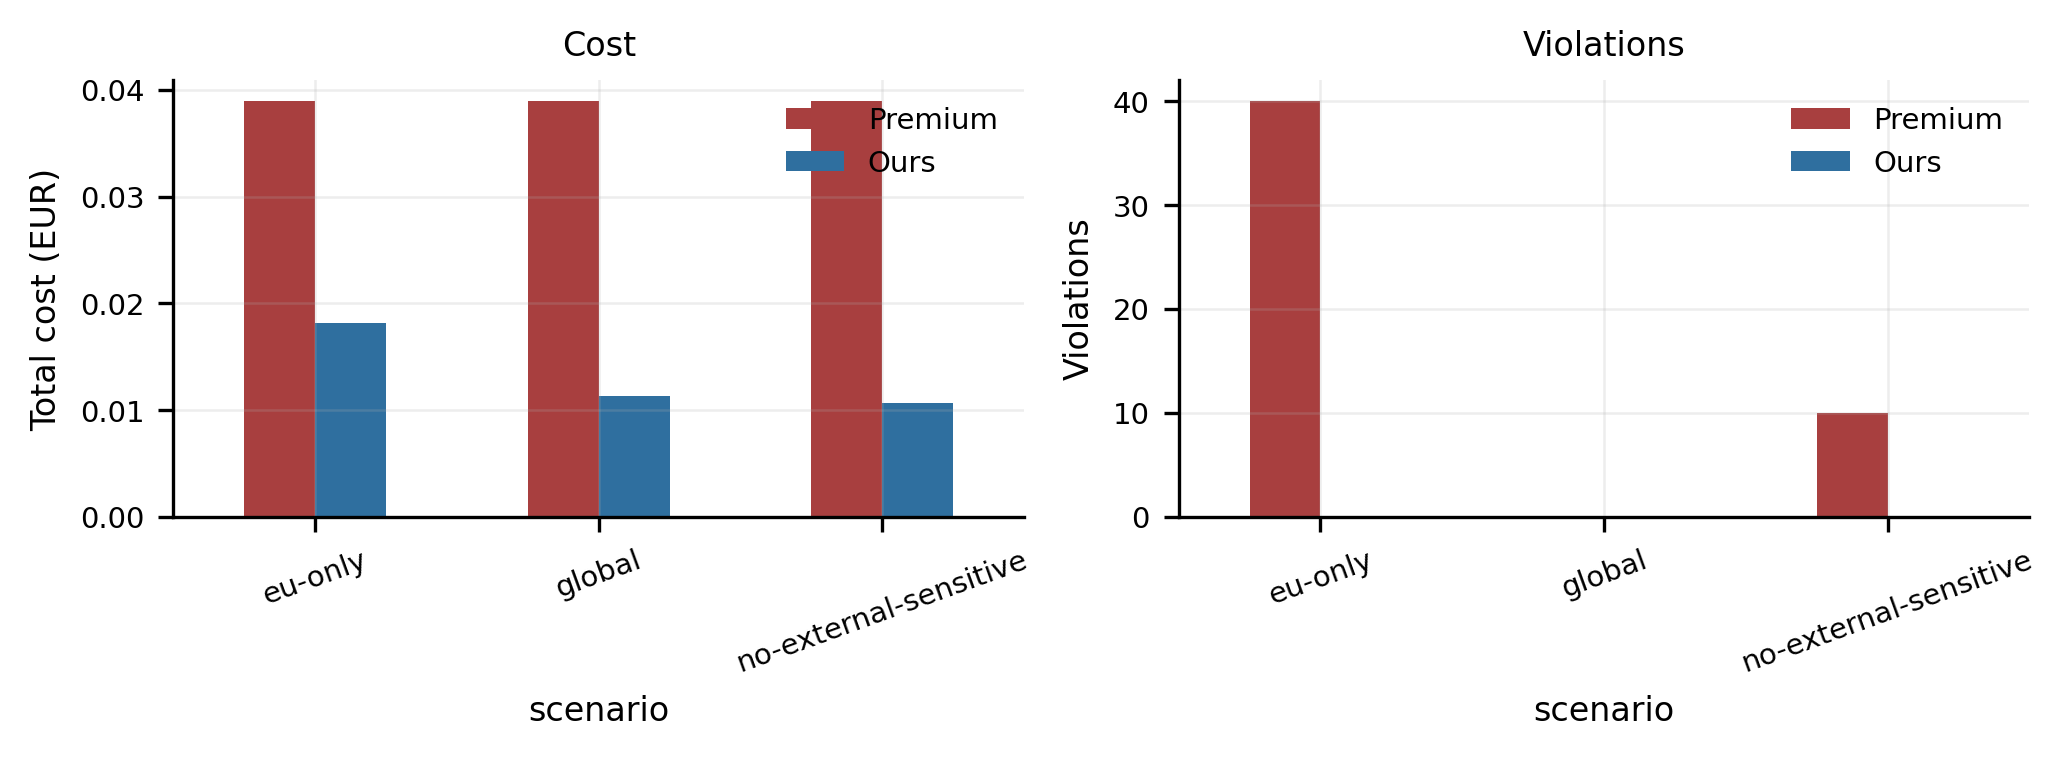
\includegraphics[width=0.95\linewidth]{fig5_sovereignty.png}
\caption{SIMULATED: declared-policy scenarios over catalog metadata and cached
routes. Zero configured-policy violations are expected from hard filtering; the
scientific question is cost and availability impact.}
\label{fig:policy}
\end{figure}

Under declared metadata, policy filtering prevents configured violations by
construction. In the EU-only scenario, premium-static violates the configured
policy on 40/40 requests, while \Ours{} serves 40/40 with zero configured-policy
violations at 0.018160 EUR and mean quality 0.86625. In the
no-external-sensitive scenario, premium-static violates 10 requests, while
\Ours{} serves 40/40 with zero configured-policy violations at 0.010691 EUR. EU
zone is a declared provider/catalog attribute; the system does not verify actual
data movement or legally certify residency.

\subsection{RQ5: Budget-Pressure Behavior}
\begin{figure}[t]
\centering
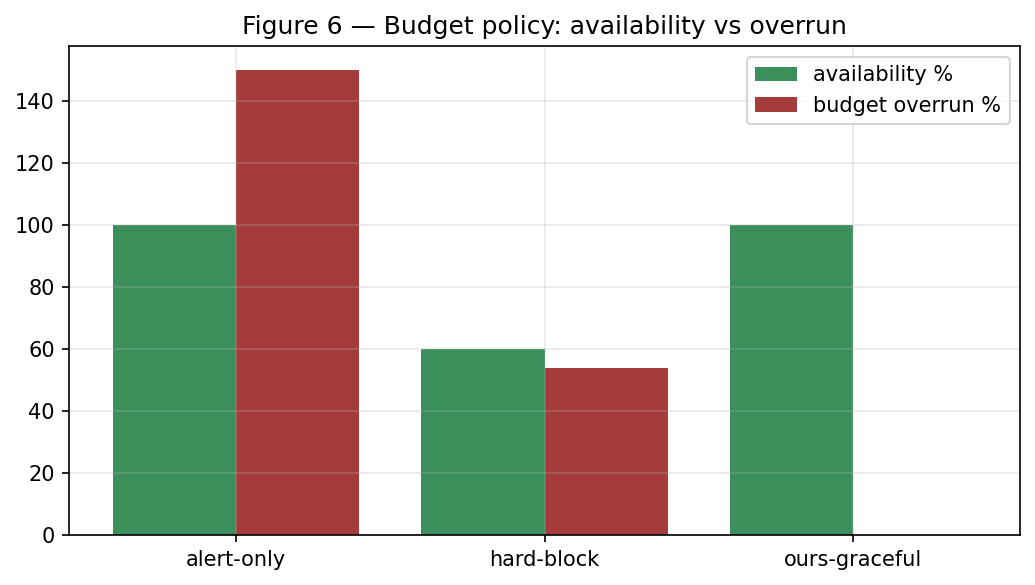
\includegraphics[width=0.95\linewidth]{fig6_budget.png}
\caption{SIMULATED: budget pressure on the analytical-agent workload.}
\label{fig:budget}
\end{figure}

In the simulated pressure scenario, alert-only serves 10/10 requests but exceeds
the configured budget by 150\%. Hard-block serves 6/10 and still exceeds the
budget by 54.03\%. The proposed graceful policy serves 10/10 with no overrun and
mean quality 0.85. This is a scenario result, not a guarantee that fallback
dominates in all deployments.

\subsection{Sensitivity, Ablation, and Stability}
\begin{figure}[t]
\centering
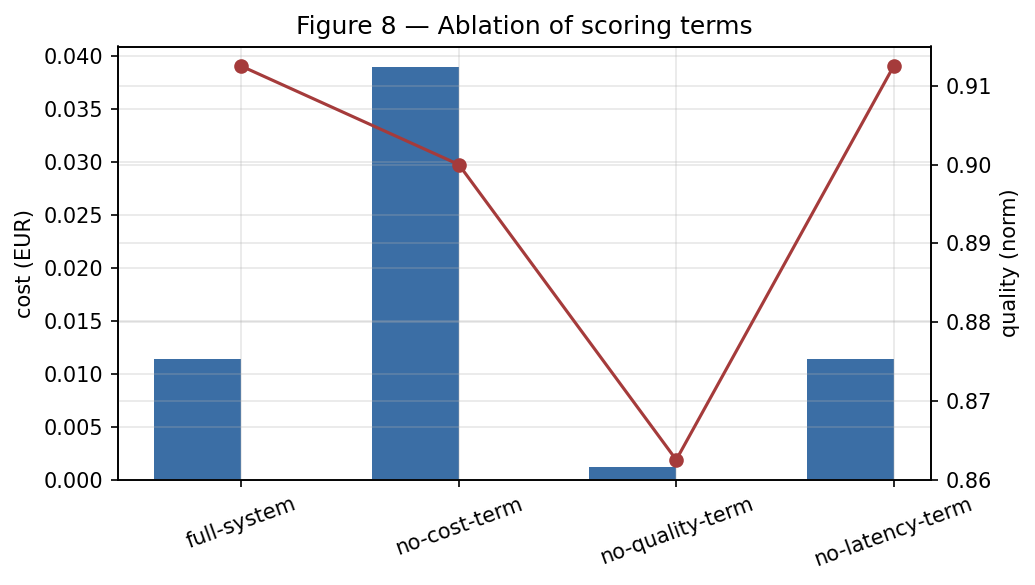
\includegraphics[width=0.95\linewidth]{fig8_ablation.png}
\caption{CACHED/SIMULATED: ablation over routing score terms.}
\label{fig:ablation}
\end{figure}

The ablation shows that removing the cost term returns the policy to the
premium-static cost (0.038930 EUR), while removing the quality term lowers cost
to 0.001213 EUR but also lowers mean quality to 0.8625. Weight sensitivity is
catalog-dependent: a policy-only least-cost variant estimates 0.003335 EUR but
uses the cheapest model for all 40 prompts and has mean quality prior 0.8000.

\begin{figure}[t]
\centering
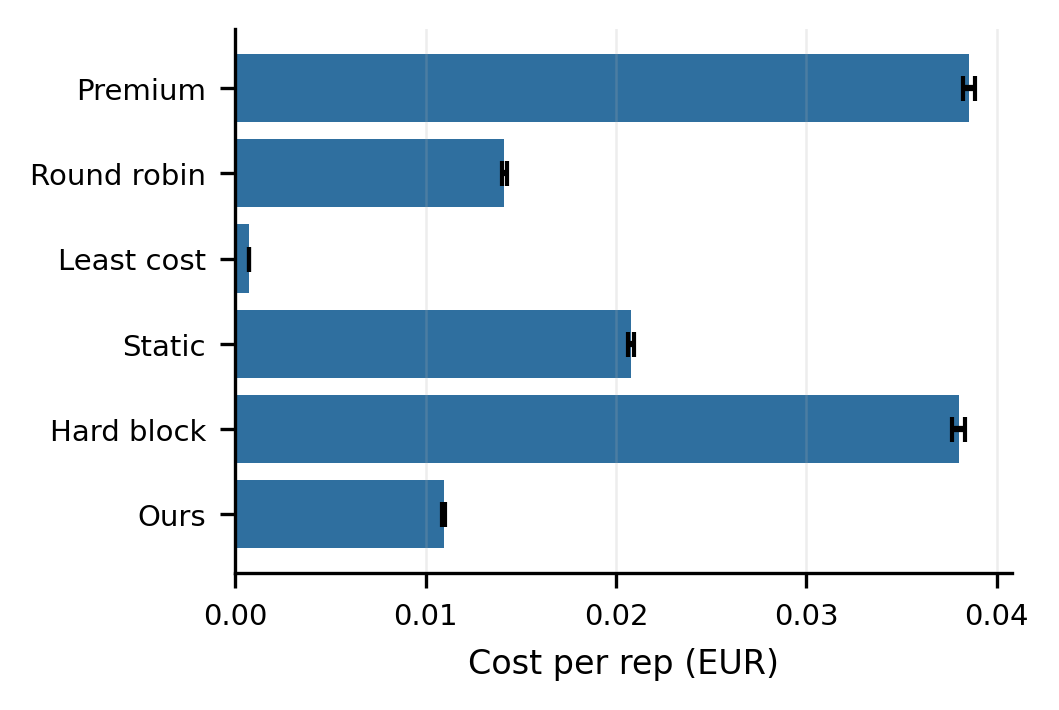
\includegraphics[width=0.95\linewidth]{fig_stats_cost.png}
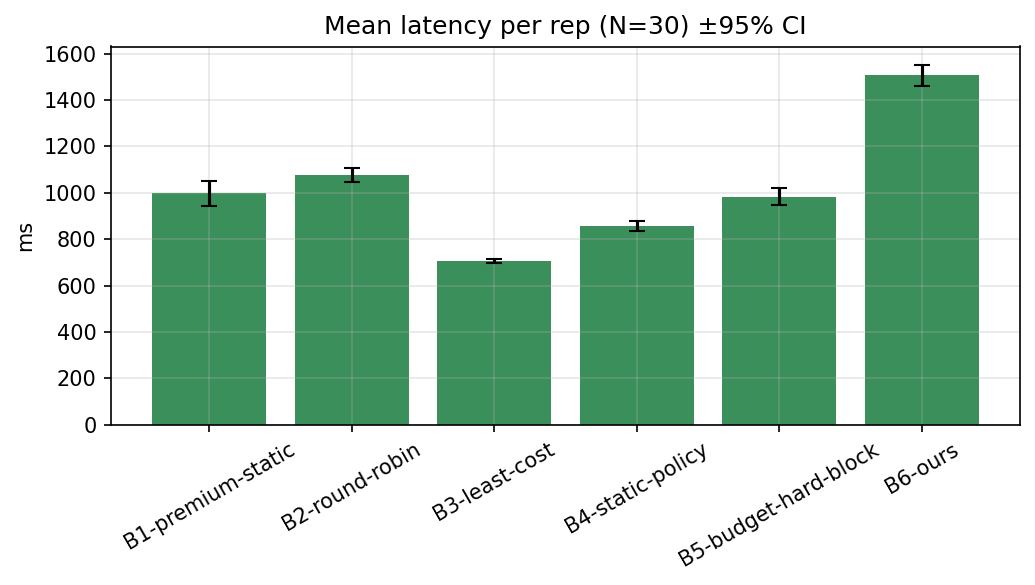
\includegraphics[width=0.95\linewidth]{fig_stats_latency.png}
\caption{MEASURED: 30 uncached repetitions over the fixed workload matrix.
Statistics indicate run-to-run stability under fixed prompts and prices, not
population-level enterprise variability.}
\label{fig:stats}
\end{figure}

Because the workload matrix and catalog prices are fixed, repeated cost
measurements have low variance. Mann--Whitney tests and large effect sizes
mainly confirm deterministic separation between policies under repeated
executions. Practical interpretation should rely on effect size, route
distribution, latency, quality, and prompt-level uncertainty.

\begin{figure}[t]
\centering
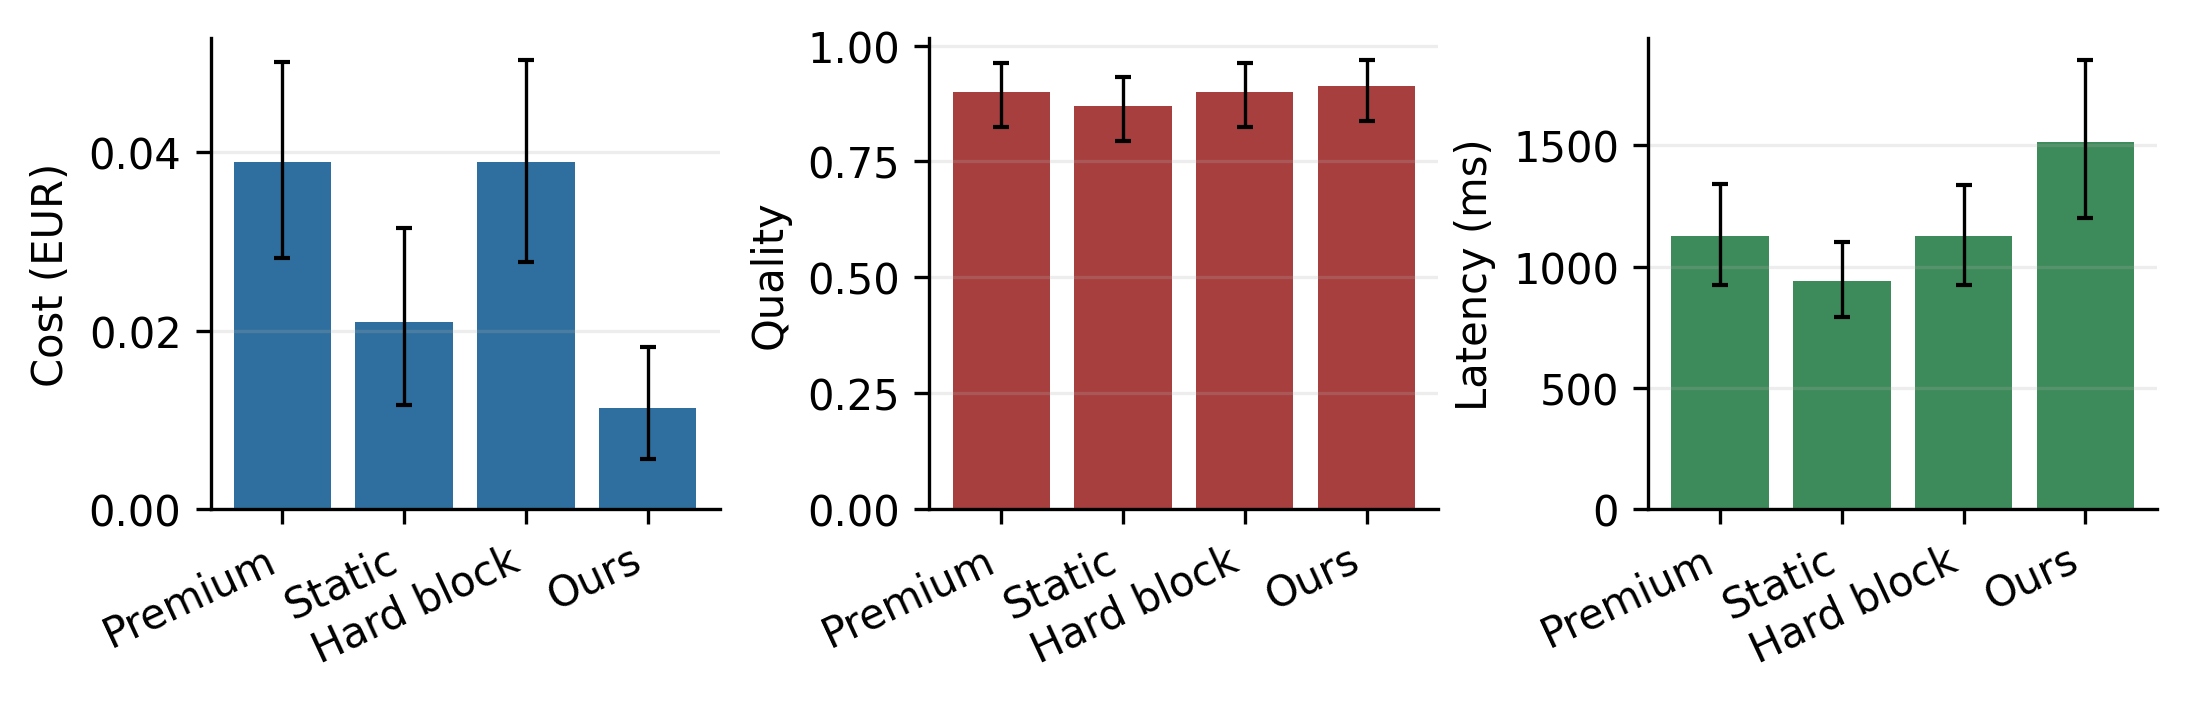
\includegraphics[width=0.95\linewidth]{fig_bootstrap_items.png}
\caption{CACHED: prompt-level bootstrap over the 40-item workload matrix.}
\label{fig:bootstrap}
\end{figure}

Prompt-level bootstrap gives a wider uncertainty view. For \Ours{}, total cost
mean is 0.011401 EUR with 95\% interval [0.005698, 0.018201], quality mean is
0.9124 [0.8375, 0.9688], and latency mean is 1512.23 ms [1200.28, 1850.13].

% =====================================================================
\section{Implementation and Evaluation Status}
\begin{table}[t]
\centering
\caption{Implementation/evaluation status.}
\label{tab:status}
\begin{tabular}{p{0.28\linewidth}ccc p{0.22\linewidth}}
\toprule
Capability & Impl. & Live & Replay/sim. & Claim level \\
\midrule
Cost attribution & \cmark & partial & \cmark & evaluated \\
Budget phase calculation & \cmark & partial & \cmark & evaluated in scenario \\
Declared-residency filtering & \cmark & partial & \cmark & evaluated as declared policy \\
Routing score & \cmark & partial & \cmark & evaluated in harness, implemented in operator \\
Envoy telemetry ingestion & \cmark & \cmark & \xmark & integration verified \\
Tetragon/shadow-AI evidence & \cmark & \cmark & \xmark & ingestion/detection verified \\
Budget fallback enforcement & \cmark & partial & \cmark & guarded, limited evidence \\
Production failover & partial & \xmark & \xmark & not claimed \\
\bottomrule
\end{tabular}
\end{table}

% =====================================================================
\section{Discussion}

\subsection{Relationship to Existing Gateways and Learned Routers}
LiteLLM and Envoy AI Gateway are complementary gateway substrates. Learned
routers are also complementary: their difficulty predictors could supply a
better quality signal inside the feasible set. The Kubernetes contribution is
the governance control plane around routing: workload ownership, CRDs,
reconciliation, namespace/application attribution, decision traces, budget
phase, and declared-policy filtering.

\subsection{Deployment Envelope and Policy Guardrails}
The approach is most appropriate for multi-tenant, governance-constrained,
mixed-difficulty workloads. Correctness-critical tasks should use premium
pinning or strict task-type guardrails. Latency-sensitive paths should constrain
candidates or increase latency weight. Single-tenant, single-provider,
low-volume deployments may not need the added control-plane complexity. The
weighted-sum policy is catalog-dependent and weight-sensitive; adaptive weights
and constrained optimization are future work.

% =====================================================================
\section{Threats to Validity}

\textbf{External validity.} The evaluation uses a bounded two-provider testbed,
four synthetic enterprise-style workloads, public GSM8K/MMLU subsets, and no
production trace. Larger traces are needed to quantify savings under production
request distributions.

\textbf{Construct validity.} Open-ended quality uses LLM judges with
weak-to-moderate inter-judge agreement, and the premium model is both baseline
and quality anchor in some analyses. Objective tasks are therefore evaluated
with exact match and reported separately.

\textbf{Internal validity.} The 30-repetition run uses the same workload matrix;
its statistics show stability under fixed prompts and prices, not independent
population samples. Prompt-level bootstrap partially addresses item uncertainty
but does not replace production traces.

\textbf{Policy validity.} Provider zone and sensitive-data suitability are
declared catalog attributes. The operator filters and reports based on those
attributes, but it does not verify actual provider data movement or legal
compliance.

\textbf{Systems validity.} Integration evidence verifies telemetry attribution,
quality job plumbing, and shadow-AI evidence ingestion in an ephemeral
Kubernetes run. Scalability, multi-cluster behavior, and production failover are
not stress-tested.

% =====================================================================
\section{Data Availability and Reproducibility}
The artifact repository contains the operator source code, Kubernetes manifests,
experiment harness, datasets, cached responses, result files, and
figure-generation scripts required to reproduce the reported analyses. Provider
credentials and secrets are not included. All paths in the paper are
repository-relative. The main analysis commands are:
\begin{verbatim}
cd experimentation
python3 scripts/analyze_results.py --results results --figures figures
python3 scripts/bootstrap_items.py --calls results/calls.csv
python3 scripts/objective_guardrail.py
python3 scripts/analyze_stats.py
\end{verbatim}

% =====================================================================
\section{Conclusion}
We presented a Kubernetes-native gateway control plane for governance-aware
routing of networked LLM applications. The operator combines declared-residency
filtering, workload attribution, budget state, cost, latency, reliability, and
quality priors to produce auditable routing decisions and reports. In a bounded
two-provider evaluation, the approach reduced cached replay cost by 70.8\%
relative to an always-premium policy, and a 30-repetition uncached run confirmed
stable cost separation with a measurable latency increase. Simulated policy
scenarios showed zero configured-policy violations under declared provider
metadata by construction, with the main question being cost and availability
under the feasible candidate set. Objective GSM8K/MMLU results showed that
aggressive cost routing can reduce correctness, motivating premium pinning or
task-type guardrails for correctness-critical workloads. Overall, the results
support governance-aware LLM routing as a practical control-plane mechanism for
making cost, policy, latency, and quality trade-offs explicit in cloud-native
LLM applications. Future work will evaluate real self-hosted GPU serving and
hosting economics.

\bibliographystyle{IEEEtran}
\bibliography{references}

\end{document}
